Supppose we have
\begin{itemize}
	\item counter-constant columns  \sourceOne{}, \sourceTwo{}, \target{},
	\item a counter-constant column \source{}\mark{},
	\item binary columns $\bit{1}, \bit{2}$,
	\item byte columns \sourceOne{}\byte{}, \sourceTwo{}\byte{},
	\item ``accumulator columns'' $\acc{1}$, $\acc{2}$,
	\item a ``power'' column \col{P},
	\item a ``counter column'' \ct{}.
	%\item[\vspace{\fill}]
\end{itemize}
%\end{multicols}
The interpreation is as follows:
\sourceOne{}, \sourceTwo{} are limbs from which we will harvest a suffix and a prefix respectively;
\sourceOne{}\byte{}, \sourceTwo{}\byte{} are the respective byte decompositions of \sourceOne{} and \sourceTwo{};
\acc{1} and \acc{2} accumulate the bytes of the desired suffix and prefix;
\target{} is a limb which we will construct the previously extracted suffix and prefix;
\source{}\mark{} is a marker for bytes in \sourceOne{};
$\bit{1}$ plateaus at \source{}\mark{};
$\bit{2}$ plateaus at $16 - \source{}\mark{}$;
$\col{P}$ is pegged to $\bit{2}$ and builds a power of $256$: it is used to left shift the suffix extracted from \sourceOne{}.

The following collection of constraints ensures the desired behaviour.
% The interpreation of the greek letters ($\alpha'$, $\beta$) is given in \ob{TODO: add figure}.
\begin{enumerate}
	\item binary plateau constraints:
	\begin{enumerate}
		\item $\plateau(\bit{1}, \source{}\mark{};\ct{})$,
		\item $\plateau(\bit{2}, 16 - \source{}\mark{};\ct{})$;
	\end{enumerate}
	\item prefix and suffix constraints:
	\begin{enumerate}
		\item $\compSuffix(\acc{1}, \sourceOne{}\byte{}, \bit{1};\ct{})$, % i.e. $\acc{1}\implies\alpha'$,
		\item $\compPrefix(\acc{2}, \sourceTwo{}\byte{}, \bit{1};\ct{})$; % i.e. $\acc{2}\implies\beta$;
	\end{enumerate}
	\item power constraint: $\power(\col{P}, \bit{2};\ct{})$;
	\item value enforcement: \If $\ct_{i} = \llargeMO$ \Then $\target_i = \acc{1}_i \cdot \col{P}_i + \acc{2}_i$.
\end{enumerate}
We encapsulate all these constraints under a single relation
\[
	\twoToOneFull
	\left(
	\begin{array}{c}
	\sourceOne{}, \sourceTwo{}, \target{};\\
	\sourceOne{}\byte{}, \sourceTwo{}\byte{};\\
	\acc{1}, \acc{2}; \col{P}; \\
	\source{}\mark{}; \bit{1}, \bit{2}; \ct{};
	\end{array}
	\right)
\]

\iffalse
\begin{figure}[h!]
\centering
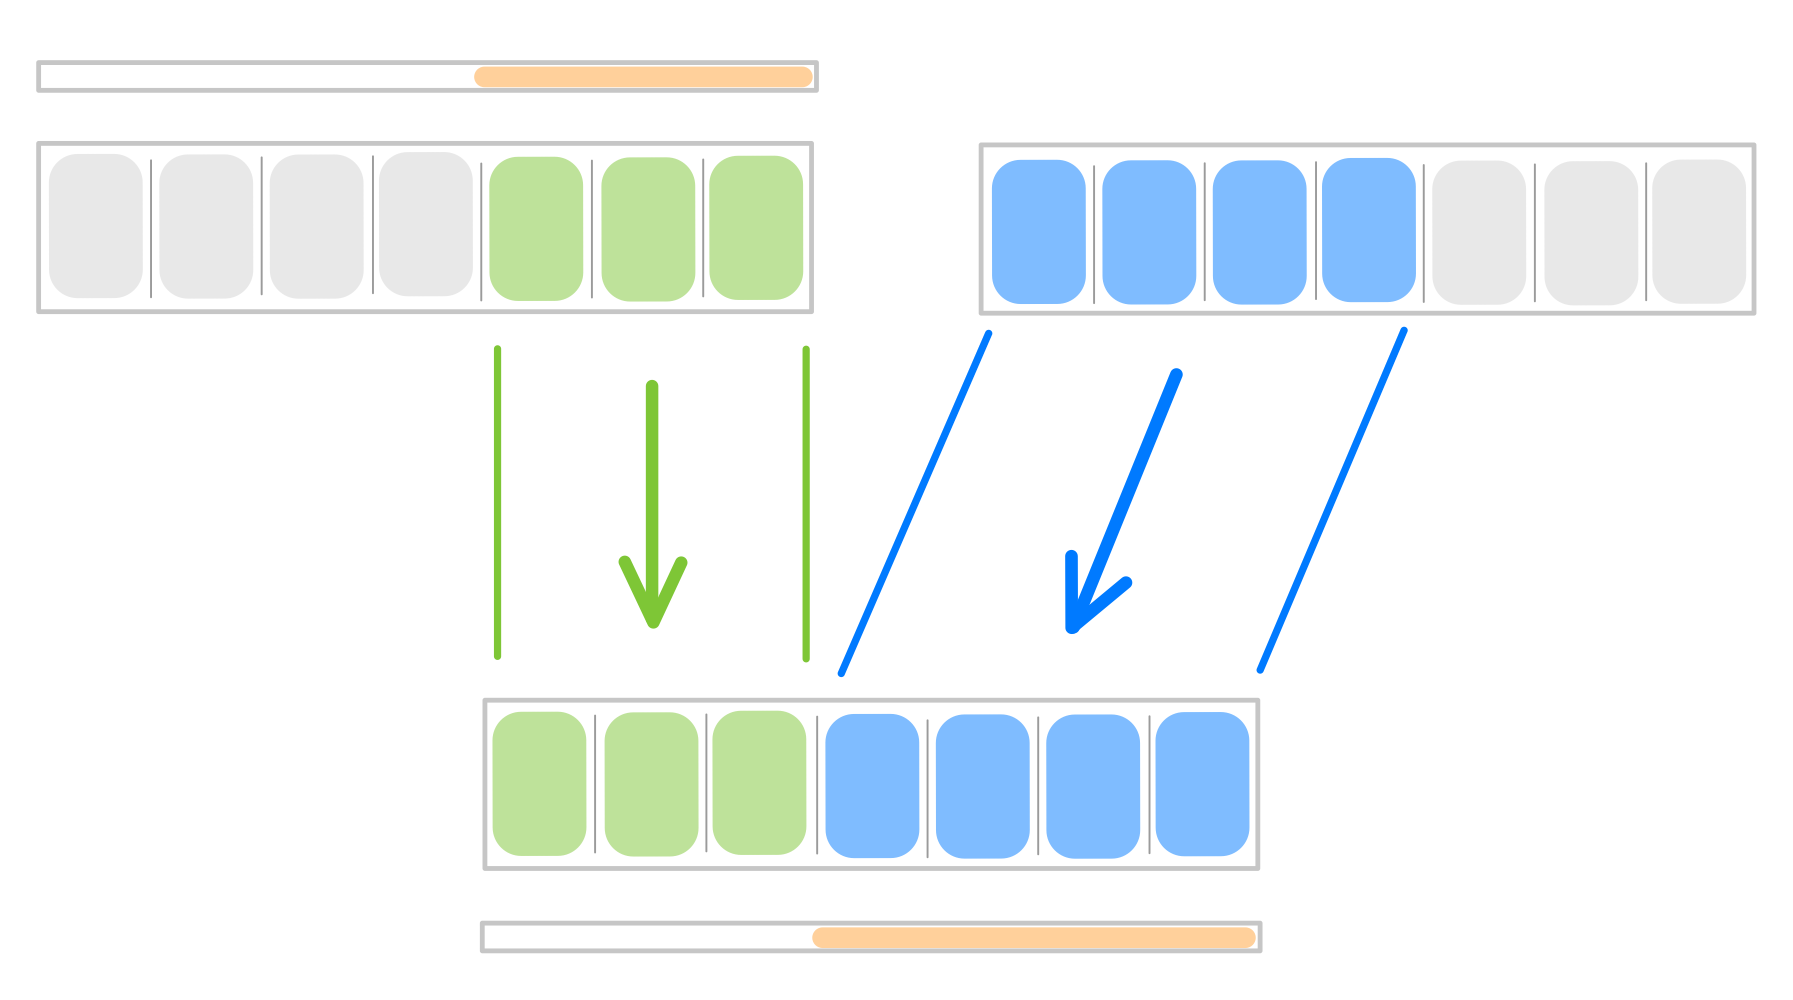
\includegraphics[width = \textwidth]{drawing/2_to_1_full}
\label{fig: one full to two}
\caption{Representation of the surgical pattern implemented by $\twoToOneFull{}$.}
\end{figure}
\fi